\chapter{Results}
\label{chap:results}
\vspace{1cm}

\section{Confined System}
\label{sec:confinedsystem}
\subsection{Edge-On Anchoring}

In Figure \ref{fig:confsnapshots} we can see a cross section of the confined system for various sizes of colloids. We can see that the imposed structure of the colloid is compatible with the imposed structure of the pore.
\begin{figure}[H]
 \centering
 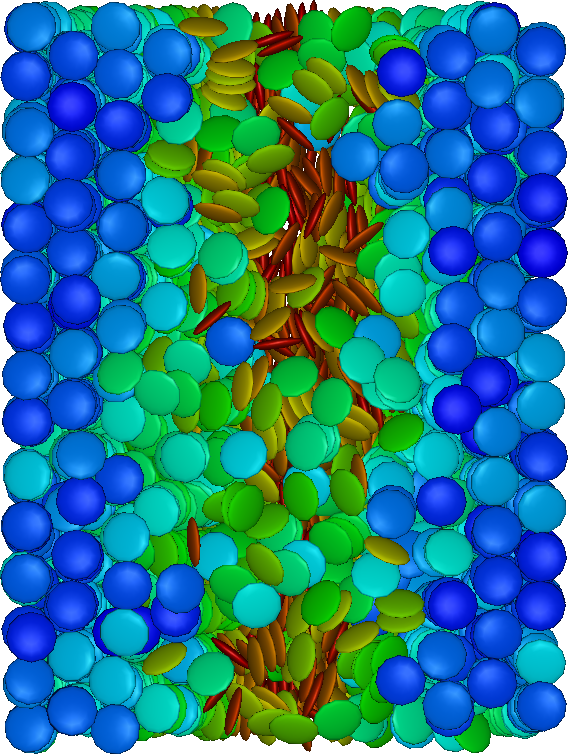
\includegraphics[width=.2\linewidth]{images/ceo_W8C8_D0.png}
 \qquad
 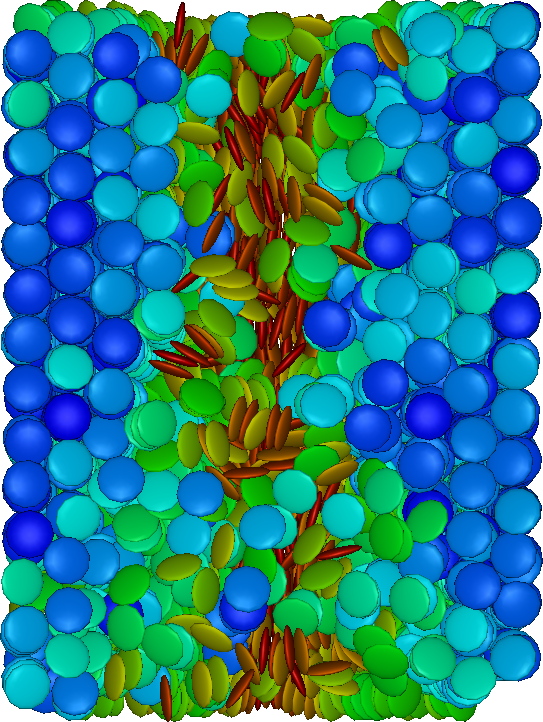
\includegraphics[width=.2\linewidth]{images/ceo_W8C8_D3.png}
 \qquad
 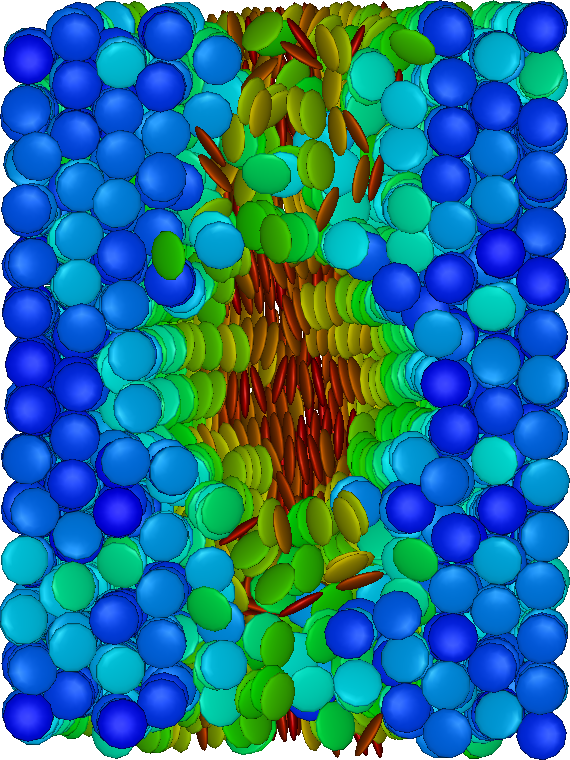
\includegraphics[width=.2\linewidth]{images/ceo_W8C8_D6.png}
 \qquad
 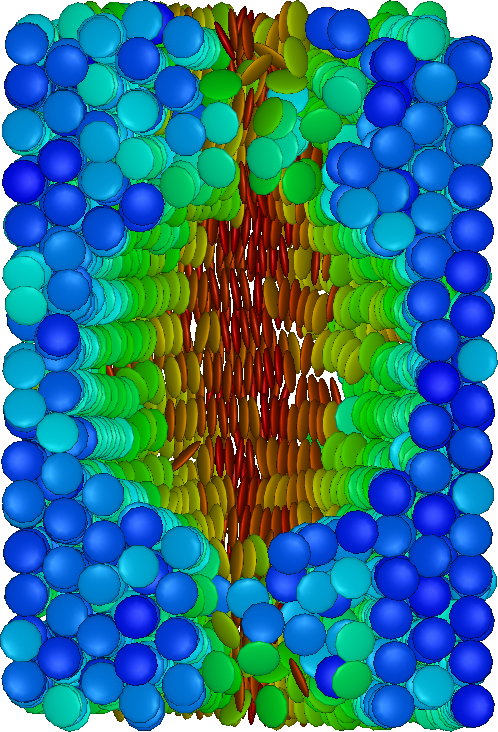
\includegraphics[width=.2\linewidth]{images/ceo_W8C8_D9.png}
 \caption{Cross sectional snapshots of the confined discotic liquid crystal system at $P^* = 50$, $T^* = 5.0$ with no colloid (far left), and with colloids of diameter $D^* \in \{3,6,9\} $. The pore diameter is $11.25\sigma_{ee}$.}
 \label{fig:confsnapshots}
\end{figure}
We can study the behaviour of the system through the various order parameters. 
Figure \ref{fig:ceoC8nemloc} shows the dependence of the local nematic order parameter on the temperature. We can see a quantized assembly of rings as found by Arne happening for every size of colloids. However, we can also see that as the colloidal size increases, the transitions happen at higher temperature and that the meta-stable plateaus appearing for smaller colloids become more sloped and the transitions become more soft. 


\begin{figure}[H]
    \centering
	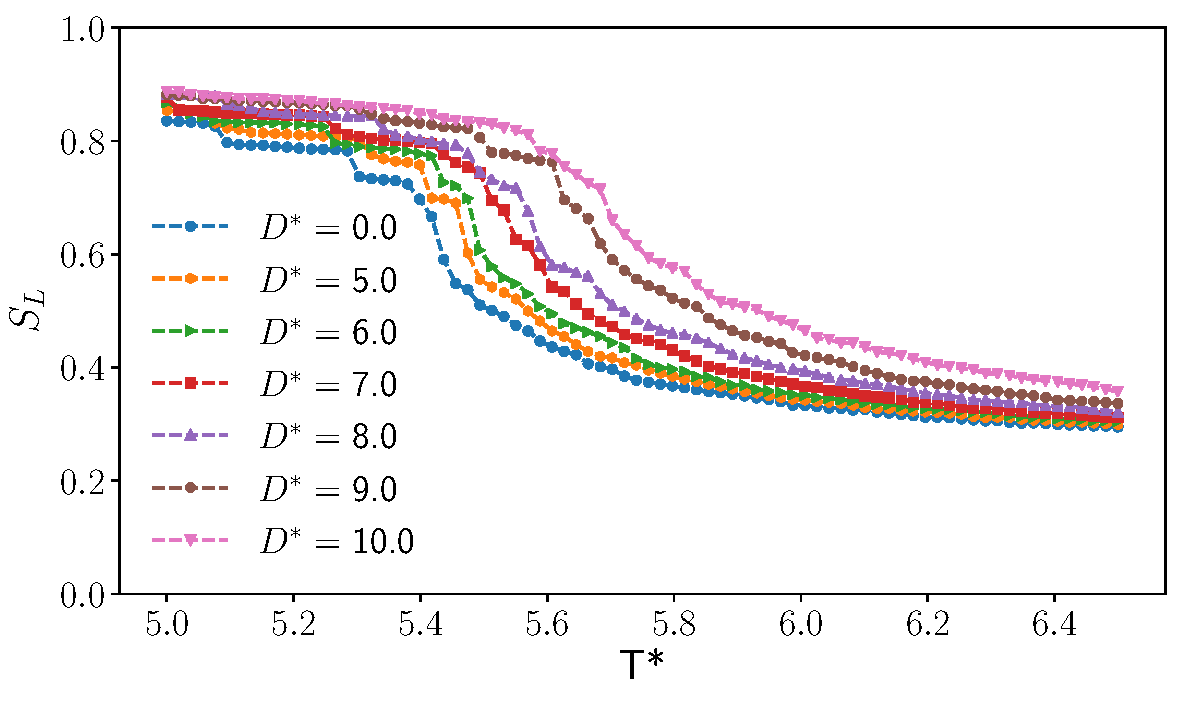
\includegraphics[width=0.8\linewidth]{plots/ceo_W8C8_nemloc.pdf}
	\caption{Dependence of the local nematic order parameter (left) and the hexagonal order parameter (right) on the temperature for confined systems with colloids of different size}
    \label{fig:ceoC8nemloc}
\end{figure}
To further study this appearance, we can look at the hexagonal order parameter which describes the columnar alignment of the rings, and the circular order parameter which describes the more general alignment along the concentric rings. 
Looking at the hexagonal order parameter we see more quantized transitions while the circular orientation
displays a similar behaviour to the local nematic order parameter which suggests that in the presence of a colloid, the circular concentric alignment of the molecules happens more continuously while the actual formation of columnar rings remainsdiscrete.  

\begin{figure}[H]
    \centering
	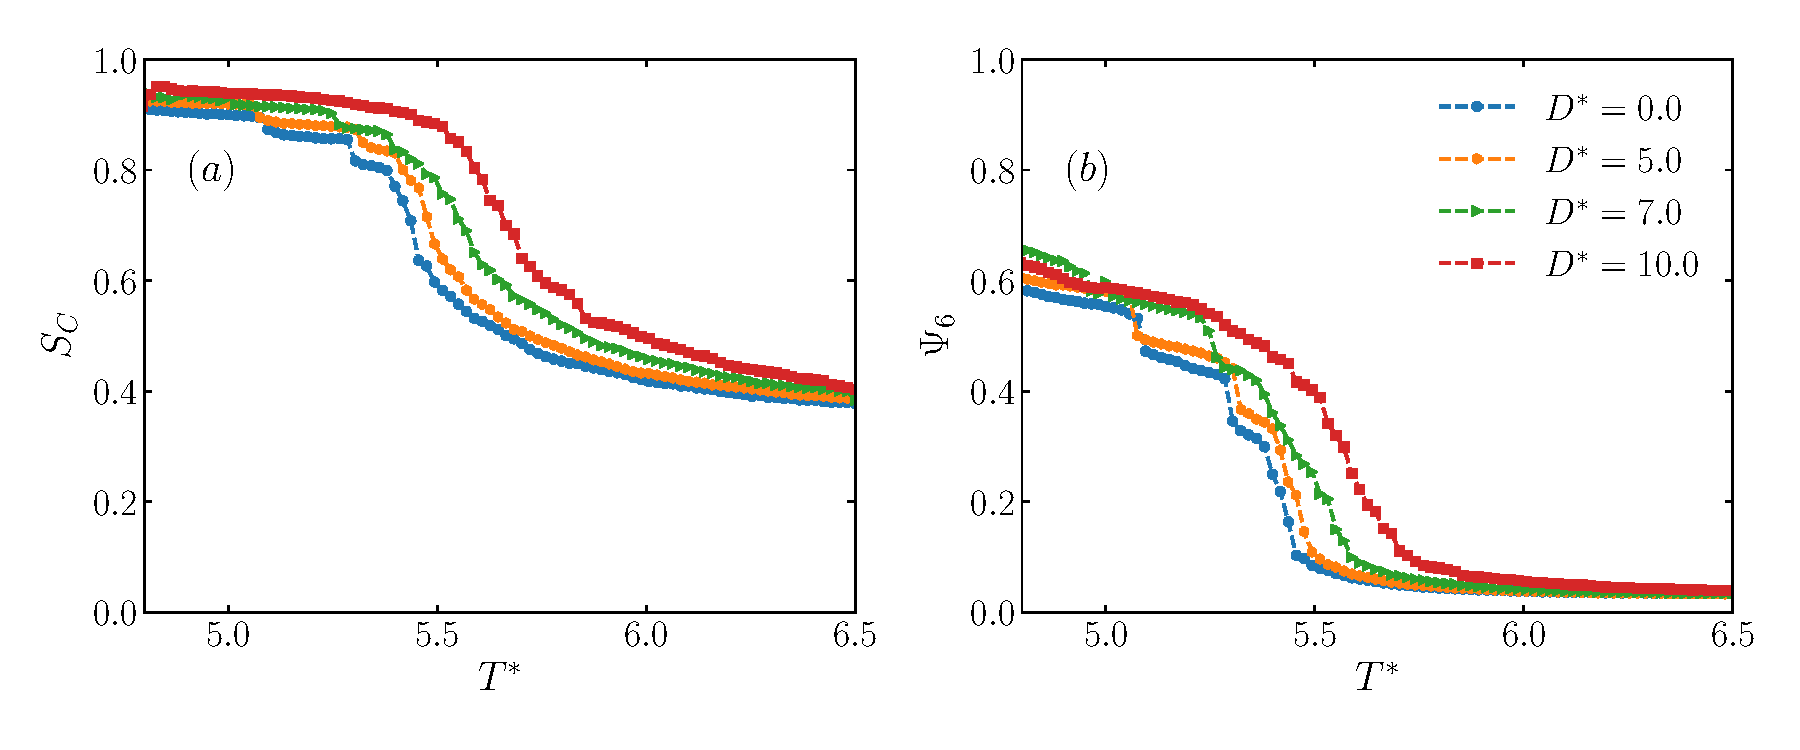
\includegraphics[width=\linewidth]{plots/ceo_W8C8_circhex.pdf}
	\caption{Dependence of the hexagonal order parameter and the circular order parameter on the temperature for confined systems with colloids of different size}
    \label{fig:ceoC8hex}
\end{figure}

If a confined system cools down even further (to $T^*< 4.5$), the inner rings start to break down, and a small domain of coaxially aligned molecules appears.
I have a feeling that the presence of a colloid would prevent that, which I would like to test in the near future. 


\label{sec:confinedsystem}
\subsection{Face-On Anchoring}
I did various simulations with various (often contradictory) results, and found out that for face-on anchoring, a high precision in the probed temperature range is very important, especially with strong colloid potentials. In the end I settled (for now) for a potential strength of $\epsilon_{\text{cf}}= 56\epsilon_{\text{ff}}$ since it produced fairly nice results.


Looking at the local nematic order parameter in function of the temperature, we see, that the nature of the transition does not change, which however is shifted towards colder temperatures, as the colloid grows in diameter.

\begin{figure}[H]
    \centering
	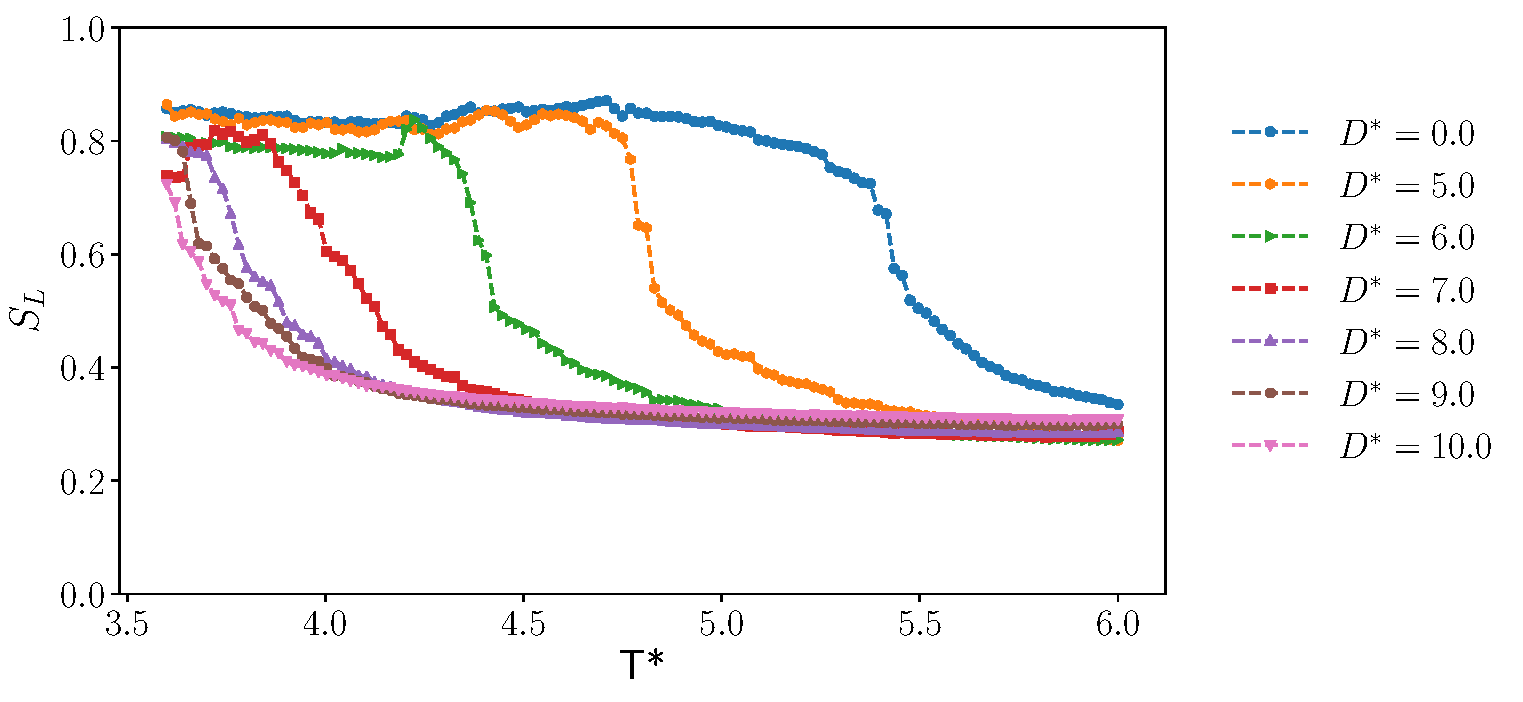
\includegraphics[width=\linewidth]{plots/cfo_W8C56_nemloc.pdf}
	\caption{Dependence of the local nematic order parameter and the hexagonal on the temperature for systems in bulk with colloids of different size}
    \label{fig:beoc32lochex}
\end{figure}
\begin{figure}[H]
    \centering
	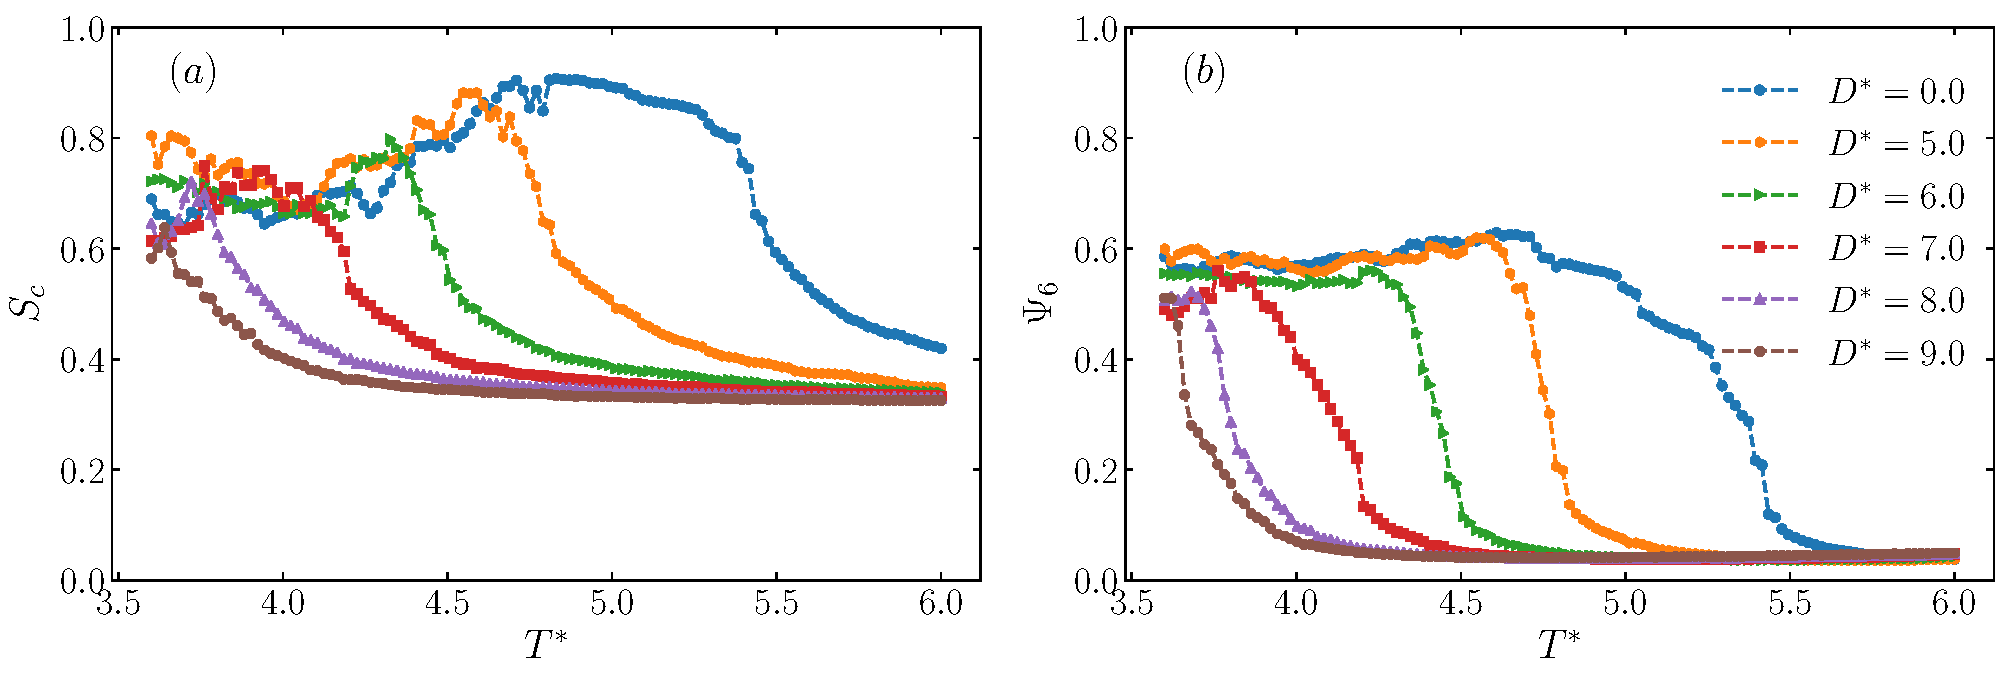
\includegraphics[width=\linewidth]{plots/cfo_W8C56_hexcirc.pdf}
	\caption{Dependence of the local nematic order parameter and the hexagonal on the temperature for systems in bulk with colloids of different size}
    \label{fig:cfohexcirc}
\end{figure}

Cooling the system even further down the inner rings break up/ never really form and the aforementioned domain of (generally) coaxially aligned particles, which can be seen by the drop in circular nematic order at lower temperatures in Figure \ref{fig:cfohexcirc}, whereas the local nematic order and hexagonal order stay fixed. If we look at the radial density, we can definitely see the formation of the concentric outer rings and can also "guess" the formation of the inner patch, in the way the become more blurred \footnote{I'm actually not really sure how to show this, since the alignment of that inner patch is not completely coaxial, but rather (sometimes very) sloped (see Fig, \ref{fig:cfosnapshots}. Also the distance between particles along the concentric planes remain $1\sigma_{\text{ee}}$ which is why probably the small peaks still appear at $r<3\sigma{\text{ee}}$ even if there are no actual rings.}.

\begin{figure}[H]
 \centering
 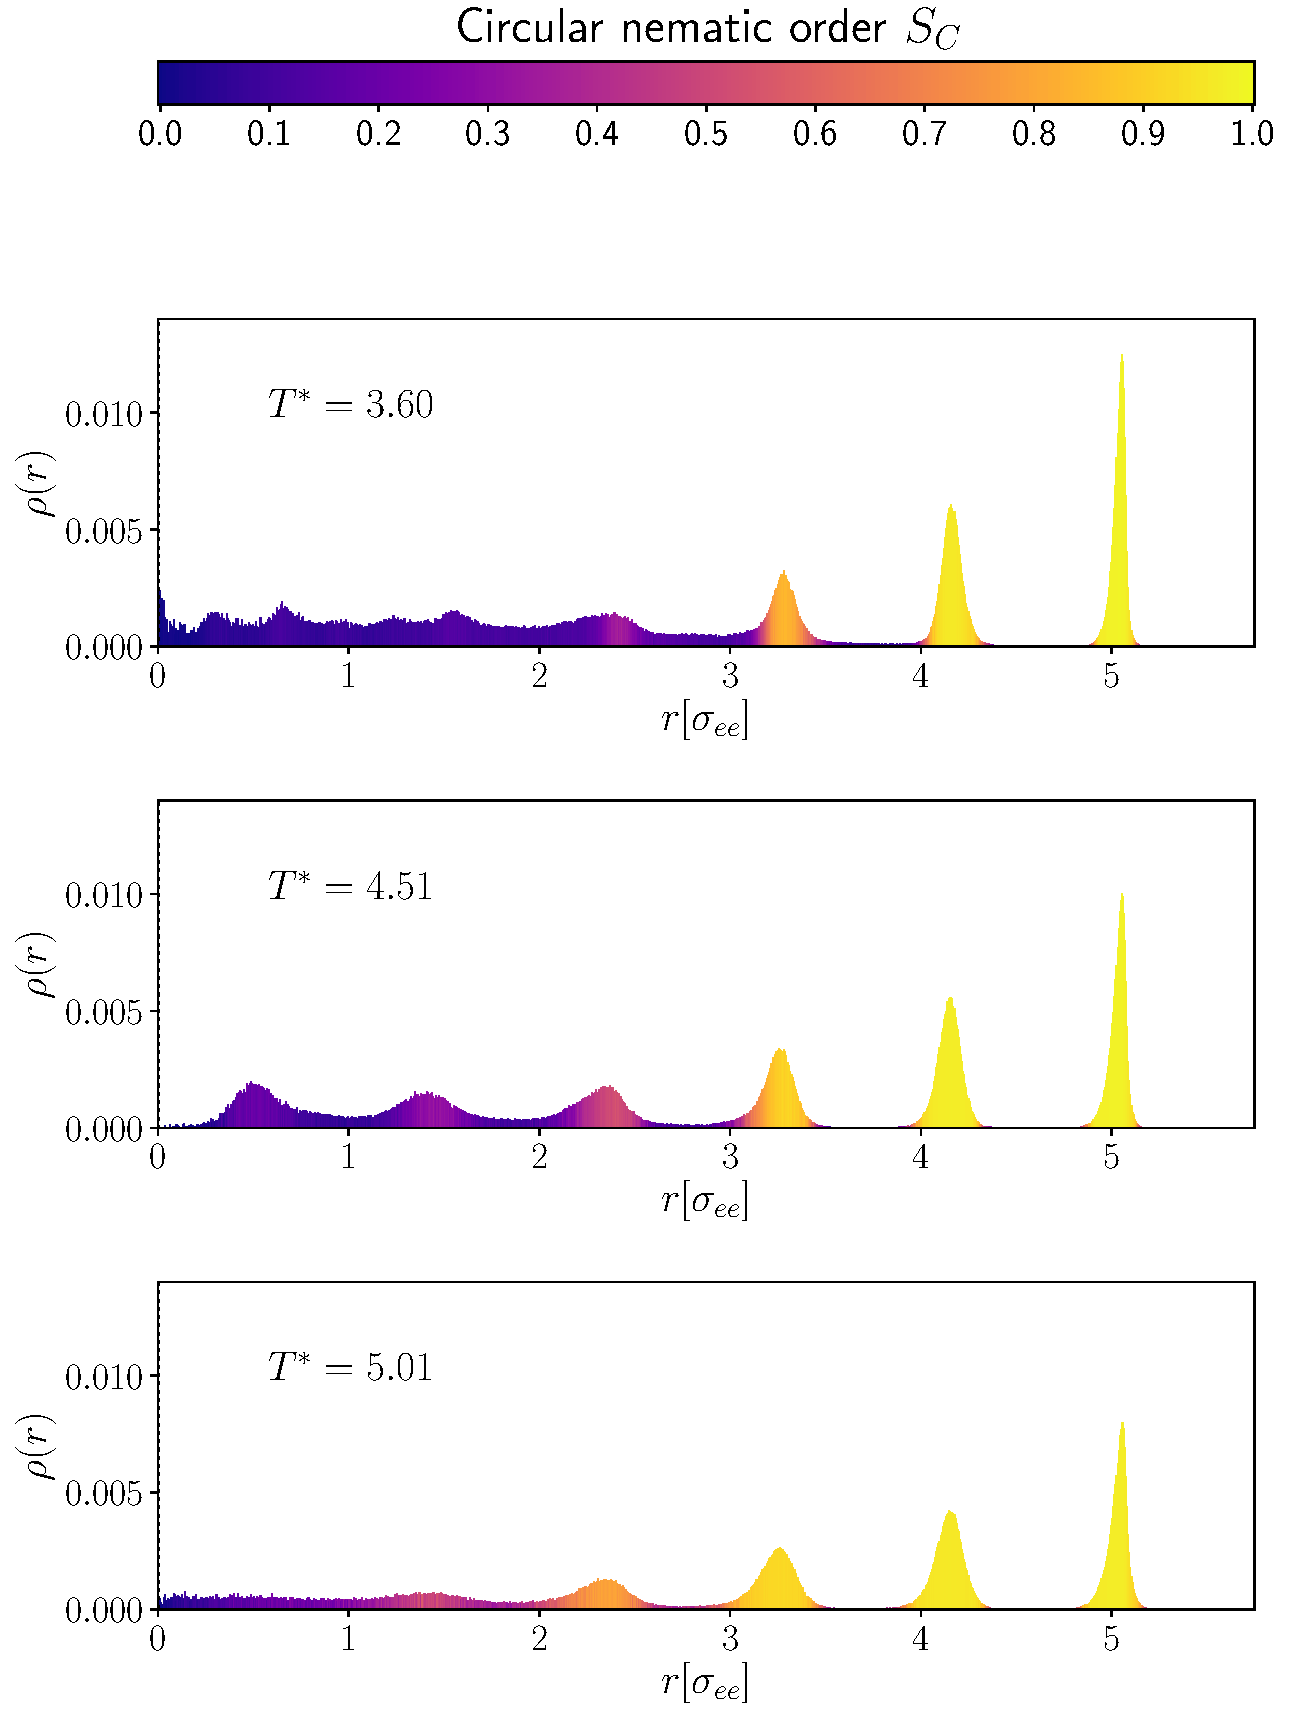
\includegraphics[width=.49\linewidth]{plots/cfo_W8C56_raddensD0.pdf}
 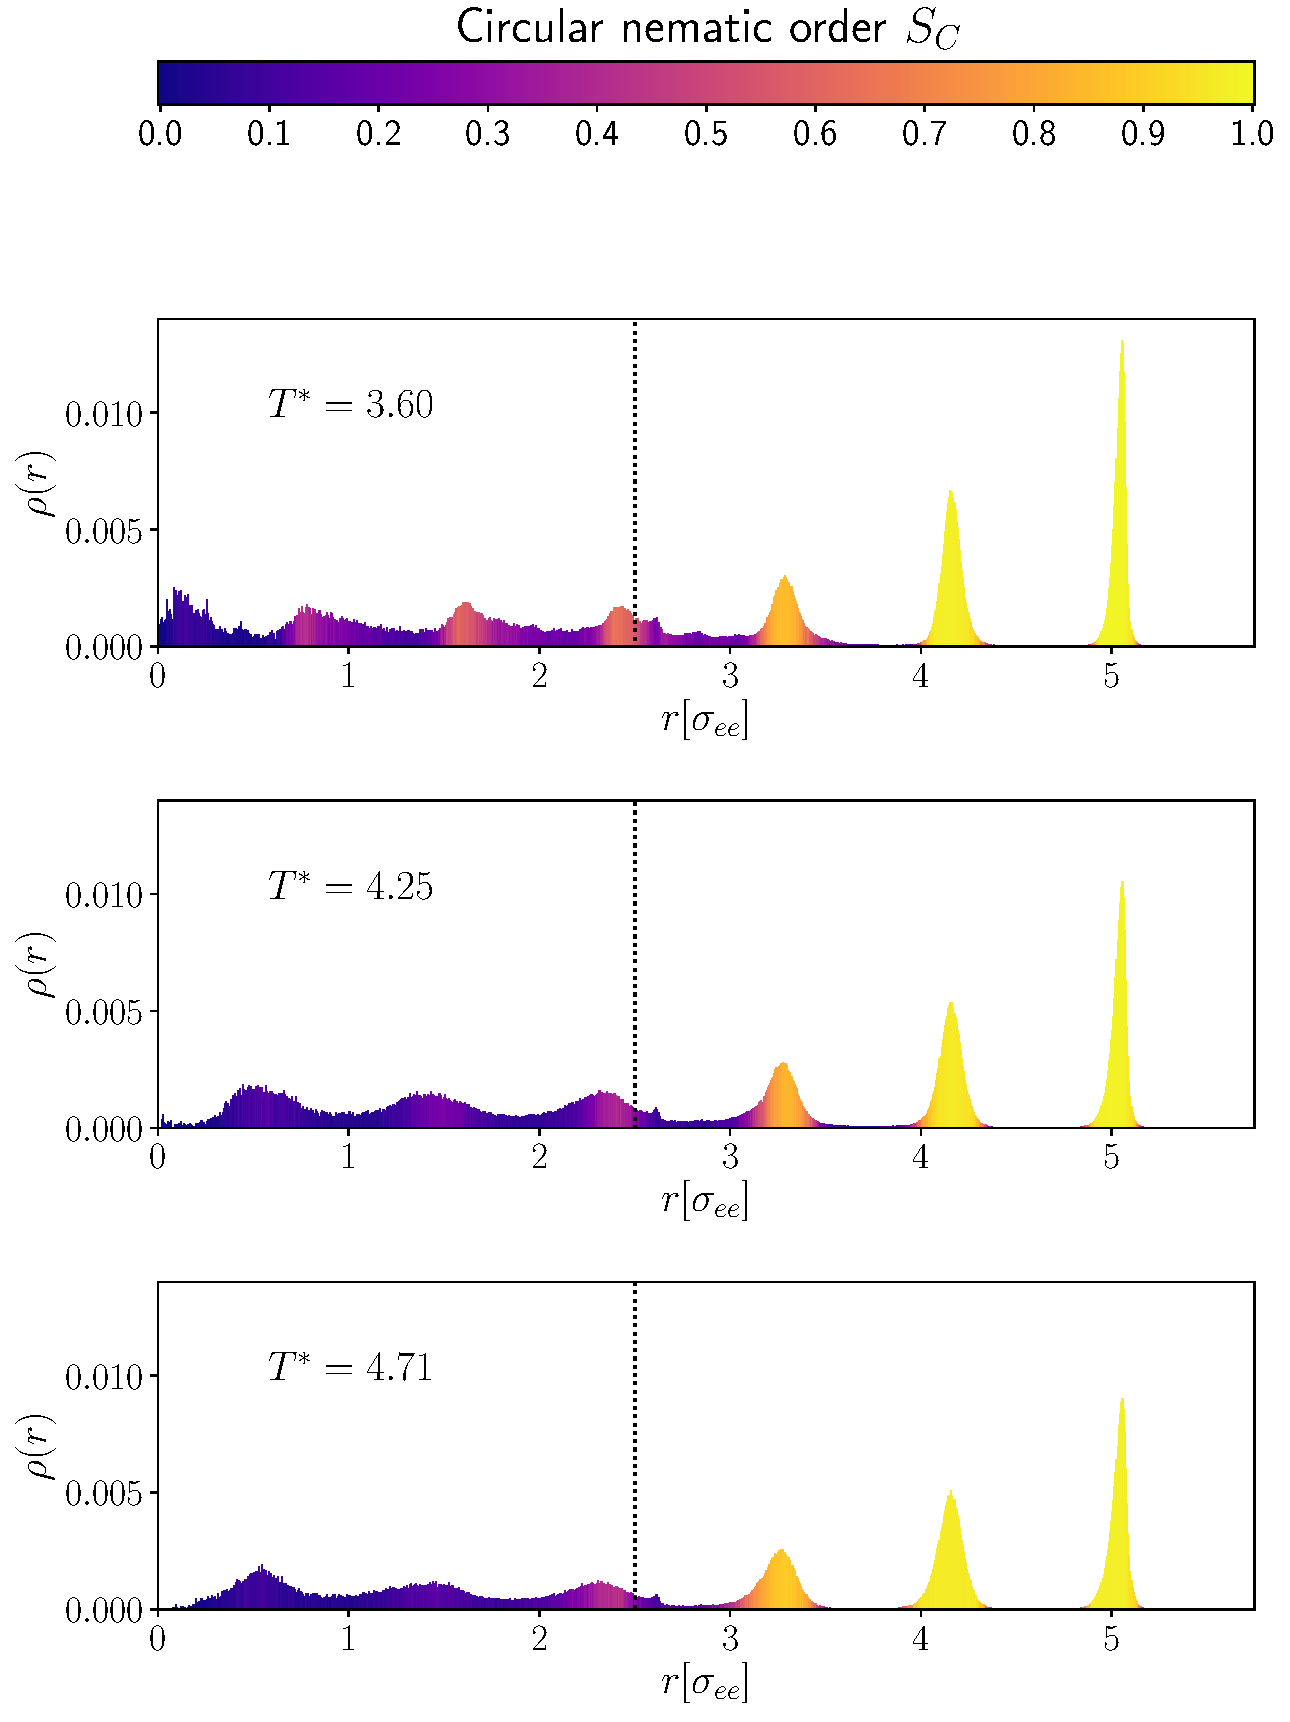
\includegraphics[width=.49\linewidth]{plots/cfo_W8C56_raddensD5.pdf}
\caption{Radial dependence of the local density and circular nematic order at different temperatures for a system without a colloid (left) and a system with a colloid of diameter $D^* = 5$ (right). The vertical dashed line represents the radius of the colloid.}
 \label{fig:bfosnapshots}
\end{figure}

\begin{figure}[H]
 \centering
 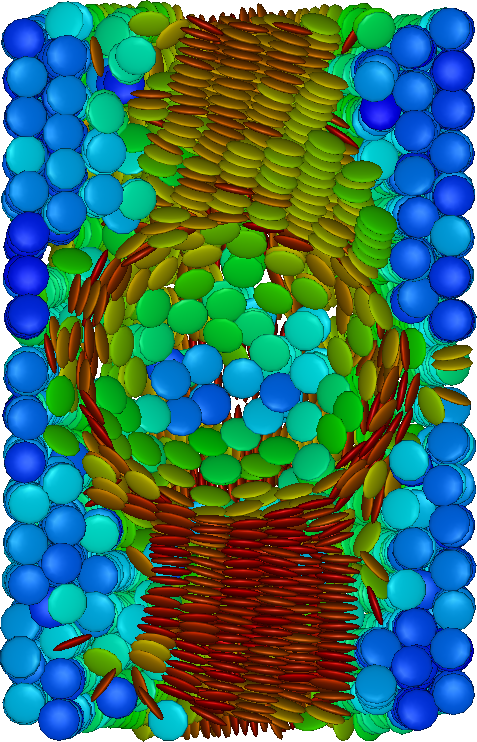
\includegraphics[width=.2\linewidth]{images/cfo_W8C56_D7.png}
\caption{Cross sectional snapshots of the confined discotic liquid crystal system at $P^* = 50$, $T^* = 3.7$ with colloids of diameter $D^*=7 $.}
 \label{fig:cfosnapshots}
\end{figure}



\section{Bulk}
\label{sec:Bulk}
To study the system in bulk we imposed periodic boundary conditions and set a colloidal particle of diameter $D^* \, [\sigma_{ee}]$ in the centre of the system. To try to avoid any small system effects due to the periodic boundary conditions, I had to simulate 10000 particles to offset the size of the colloid, which ranges from $1$ to $10$.\footnote{One possible way to artificially reduce the necessary particle number is to choose a different shape for the simulation box, e.g. a truncated octahedron, that has better sphericity. However, I suspect the box would have to be a regular polyhedron, which may be a disadvantage due to the irregular shape of the particles.} Most effects start appearing only for colloids of diameter $D^* \geq 6$. This takes quite some time (between one and two weeks for one batch of simulations) since the range of temperatures has to be fairly precise so as to avoid any weird effects happening, and the number of performed equilibration steps needs to be increased with the number of particles. therefore the results here are not as complete as I would prefer. In particular the plots of the (global) nematic order parameter in function of the temperature are very noisy, due to the appearance of locally aligned groups of molecules. This could be solved with an even longer run-time, and maybe a few optimizations in the code, which of course would take even longer to run.

\subsection{Edge-On Anchoring}

\begin{figure}[H]
 \centering
 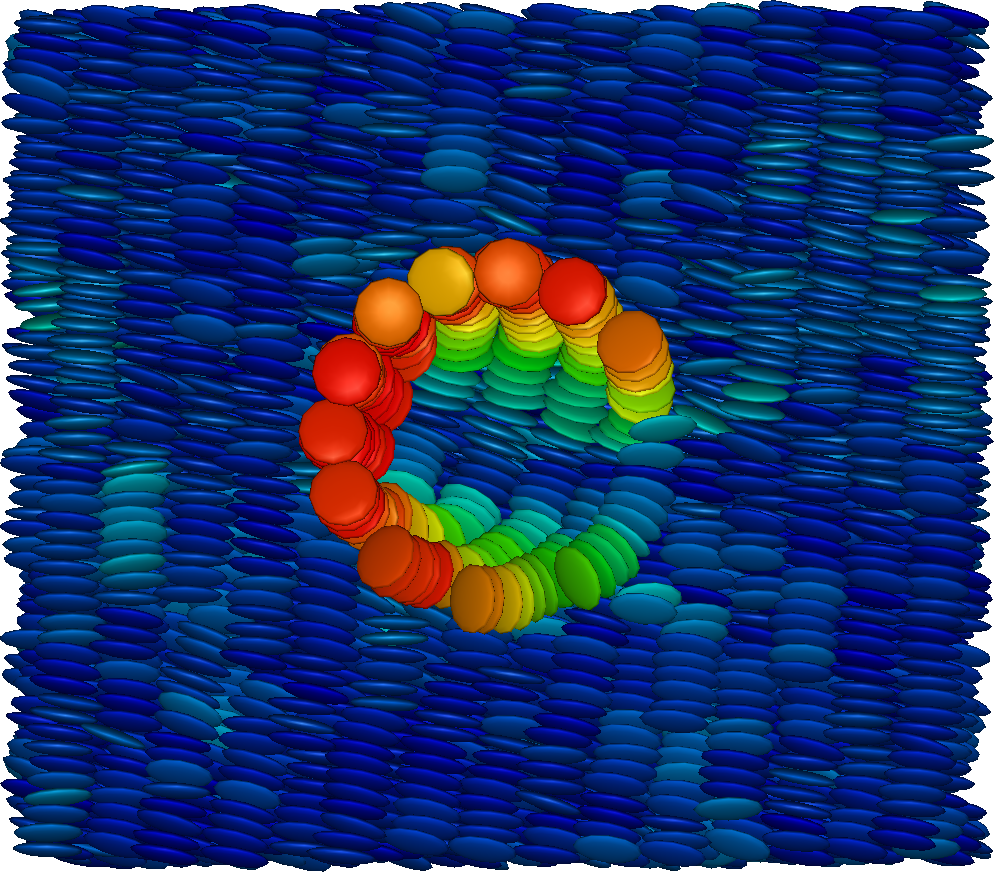
\includegraphics[width=.4\linewidth]{images/beo_C32_D5.png}
 \qquad
 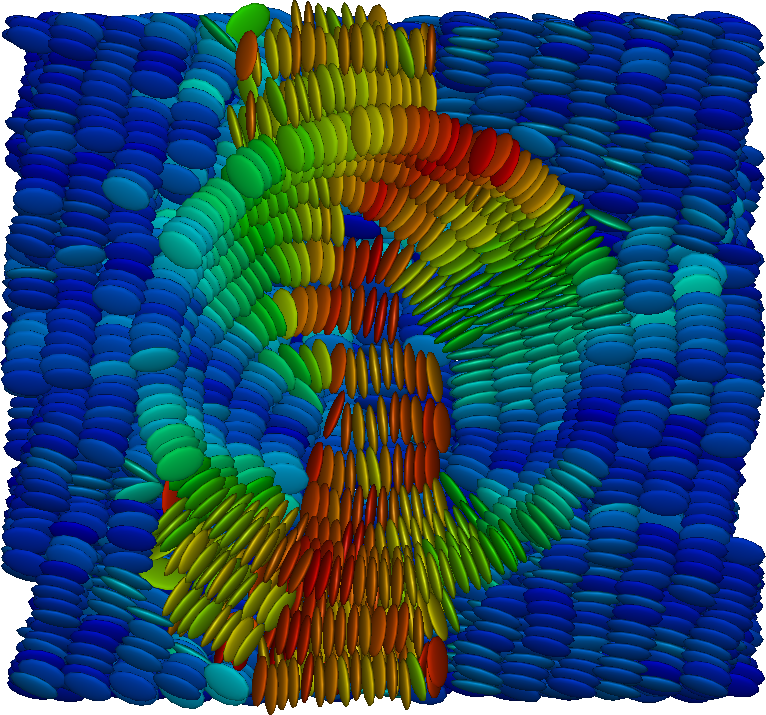
\includegraphics[width=.4\linewidth]{images/beo_C32_D9.png}
\caption{Cross sectional snapshots of the bulk discotic liquid crystal system at $P^* = 50$, $T^* = 4.6$ with colloids of diameter $D^* \in \{5,9\} $.}
 \label{fig:beosnapshots}
\end{figure}


Imposing edge-on anchoring on the colloid we can see in Fig. \ref{fig:beoc32lochex} that the phase transition becomes continuous with the introduction of the colloid. Whereas the bulk system without a colloid displays a first order transition the introduction of the colloid smoothens the transition, giving it a more gradual progression. We can also see that the magnitude og the order parameters in the columnar phase decrease with respect to the colloid size, which is probably due to the layer of discotic particles around the colloid at most temperatures and colloid sizes.
\begin{figure}[H]
    \centering
	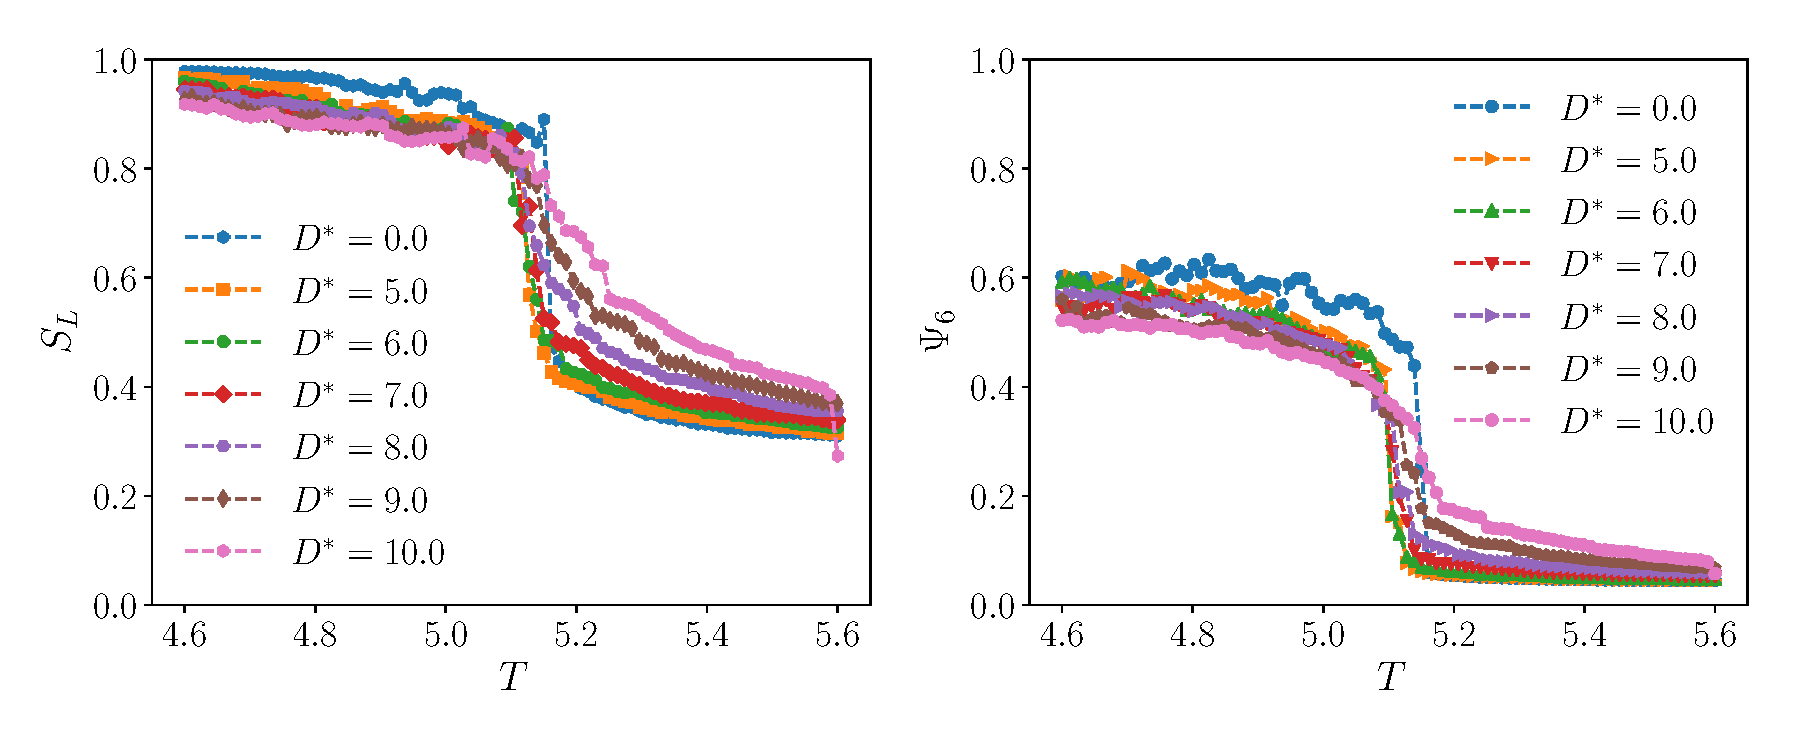
\includegraphics[width=\linewidth]{plots/beo_c32_lochex.pdf}
	\caption{Dependence of the local nematic order parameter and the hexagonal on the temperature for systems in bulk with colloids of different size}
    \label{fig:beoc32lochex}
\end{figure}

If we look at the local radial density in Figure 6 we can see at least one distinct layer of particles near the colloid forming. For the larger colloids we can see the formation of distinct layers that form in the early stages of the columnar phase that start breaking up at lower temperatures due to the tendency of alignment towards the nematic director.
\begin{figure}[H]
    \centering
	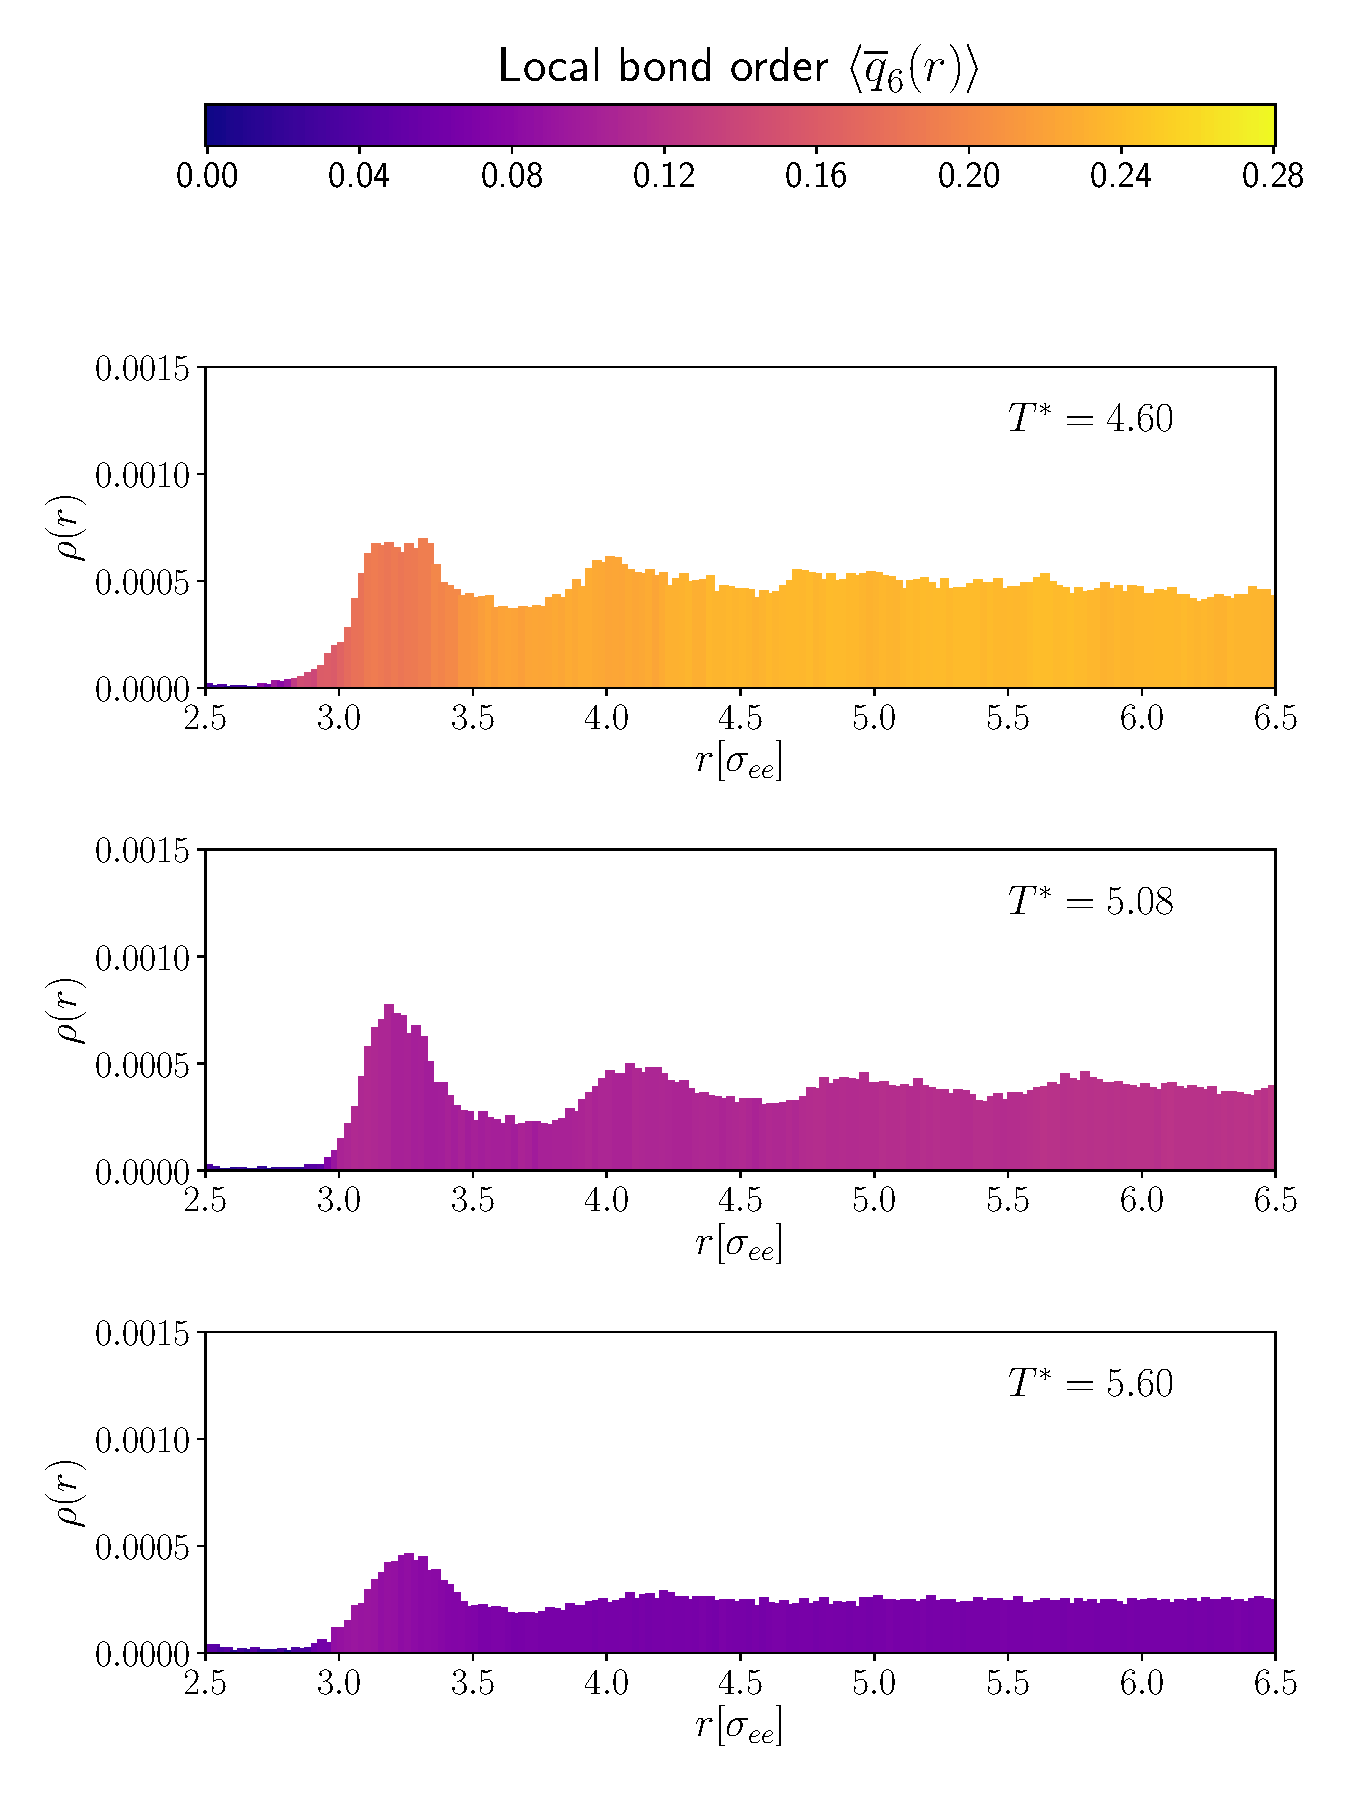
\includegraphics[width=0.49\linewidth]{plots/beo_C32_raddensD5.pdf}
	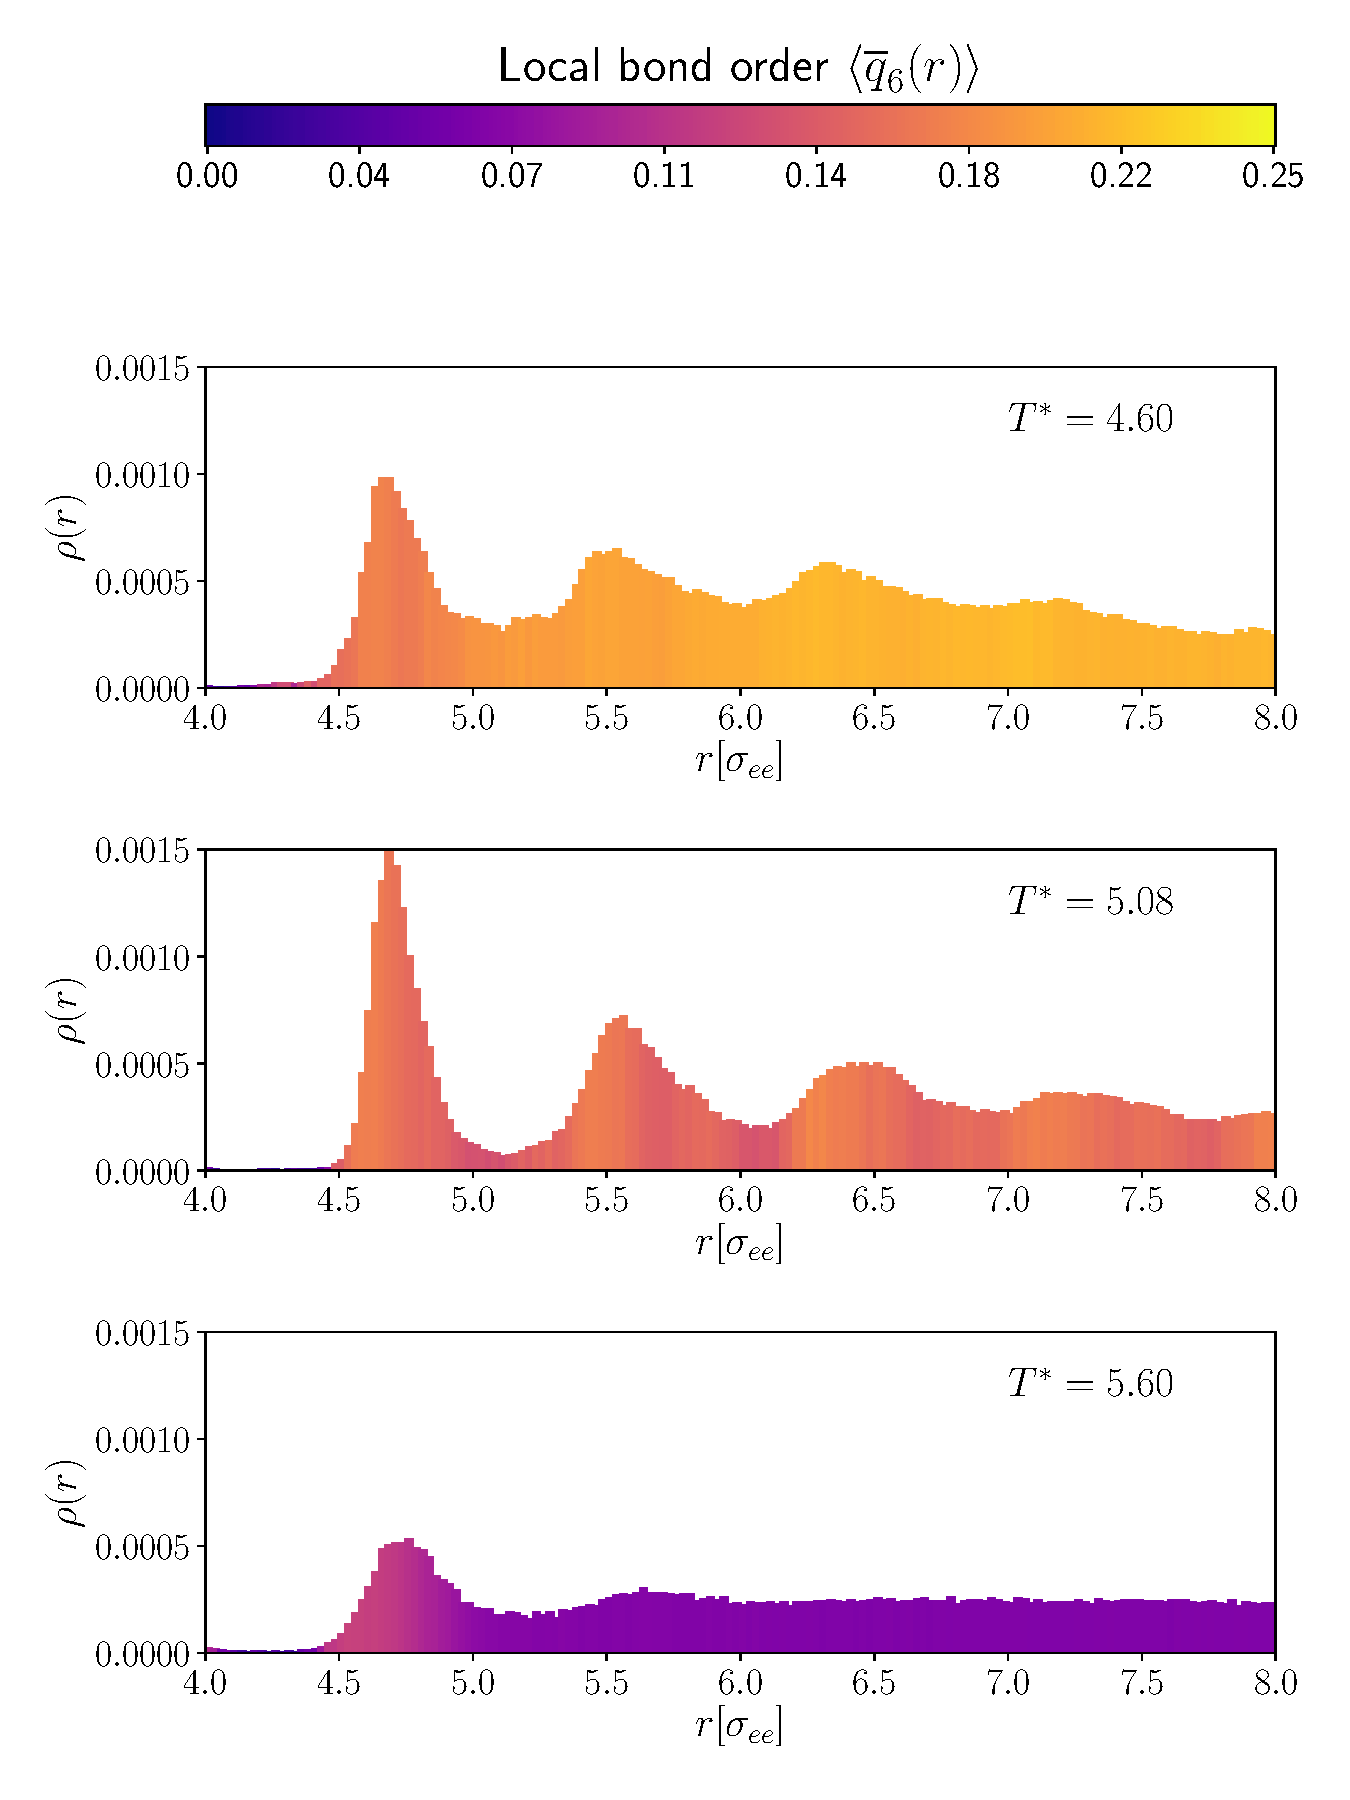
\includegraphics[width=0.49\linewidth]{plots/beo_C32_raddensD8.pdf}
	\caption{Radial dependence of the local density and bond orientational order parameter $ \overline{q}_6$ at different temperatures for a colloid of size $D^* =  5$ (left) and $D^* = 8$ (right)}
    \label{fig:beoc32nemloc}
\end{figure}


\subsection{Face-On Anchoring}


\begin{figure}[H]
 \centering
 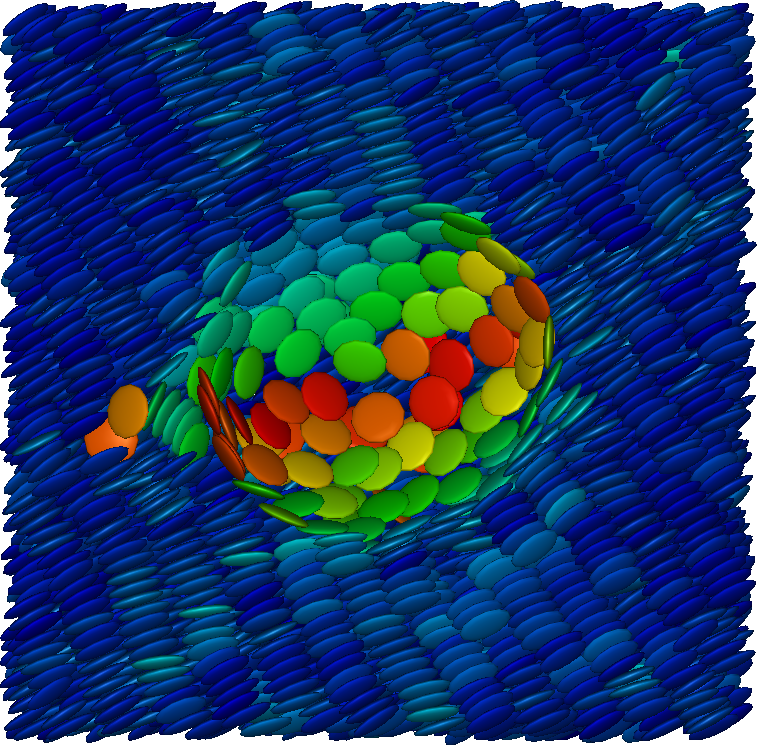
\includegraphics[width=.4\linewidth]{images/bfo_C80_D6.png}
 \qquad
 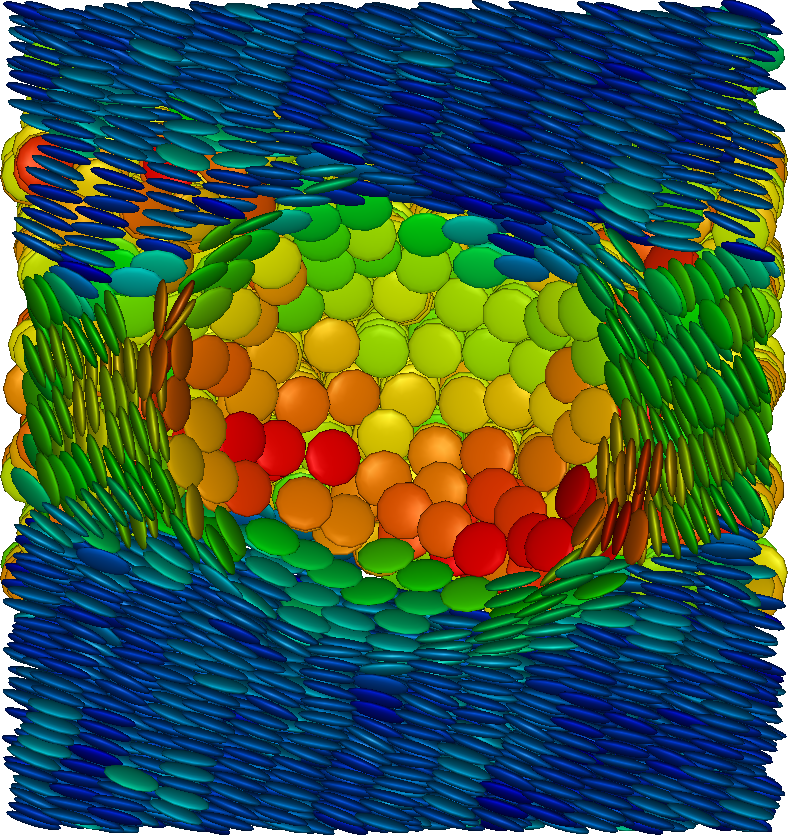
\includegraphics[width=.4\linewidth]{images/bfo_C80_D8.png}
\caption{Cross sectional snapshots of the bulk discotic liquid crystal system at $P^* = 50$, $T^* = 4.5$ with colloids of diameter $D^* \in \{6,8\} $. The colloid potential strength is $\epsilon_{\text{cf}}= 80$. }
 \label{fig:bfosnapshots}
\end{figure}

To study the face-on anchoring I did simulations at different potential strengths, yielding different results.

\subsubsection{Potential strength $\epsilon_{\text{cf}}= 32\epsilon_{\text{ff}}$}
At a potential strength of $\epsilon_{\text{cf}}= 32\epsilon_{\text{cf}}$ there is not much to be seen. The introduction of a colloid does not seem to disturb the system very much, except for a little of the phase transition temperature. Even for the large colloids the nematic order parameter tends towards $1$, which suggests that no layers of molecules form around the colloid. However, due to the slightly higher transition temperature, the colloid probably serves as some sort of nucleating agent. 
\begin{figure}[H]
    \centering
	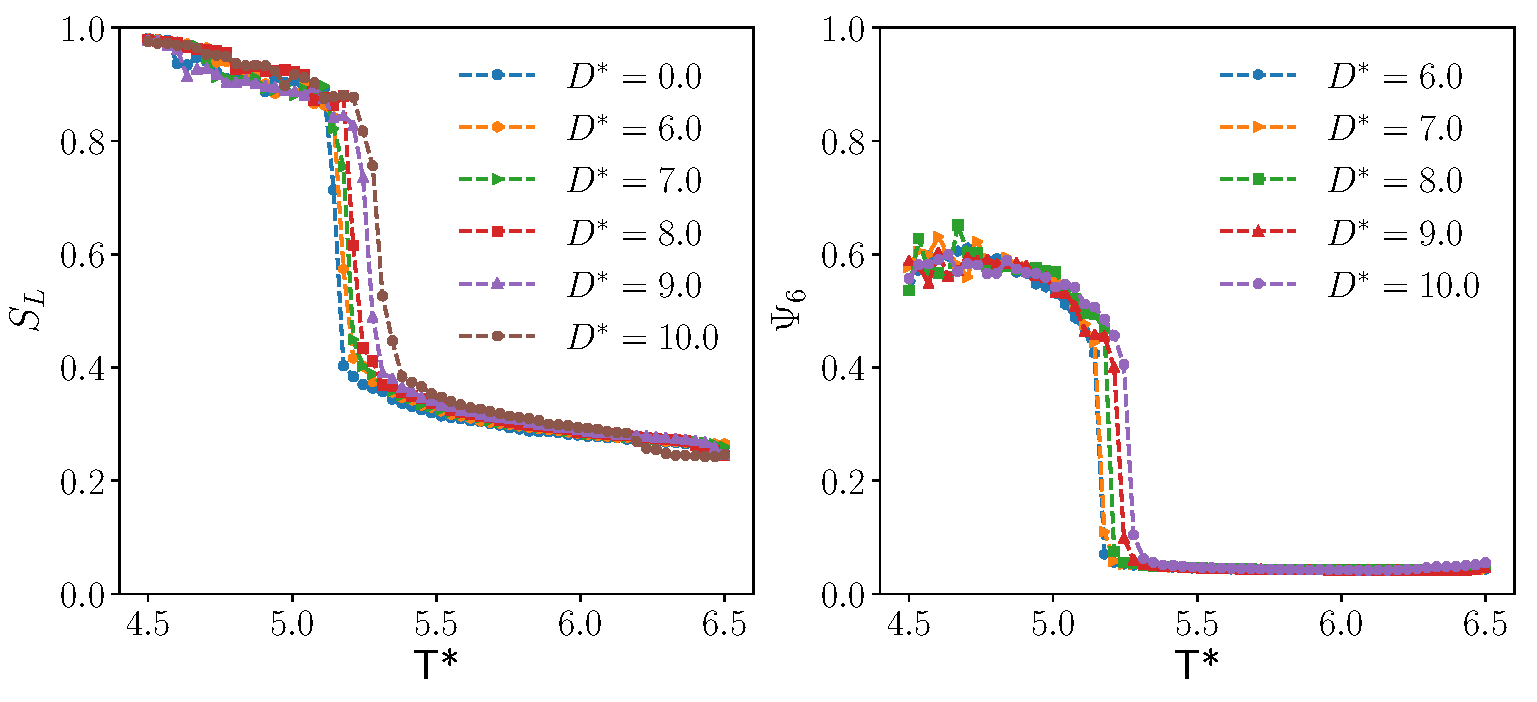
\includegraphics[width=\linewidth]{plots/bfo_C32_nemhex.pdf}
	\caption{Dependence of the local nematic order parameter and the hexagonal on the temperature for systems in bulk with colloids of different size}
    \label{fig:beoc32lochex}
\end{figure}
\begin{figure}[H]
    \centering
	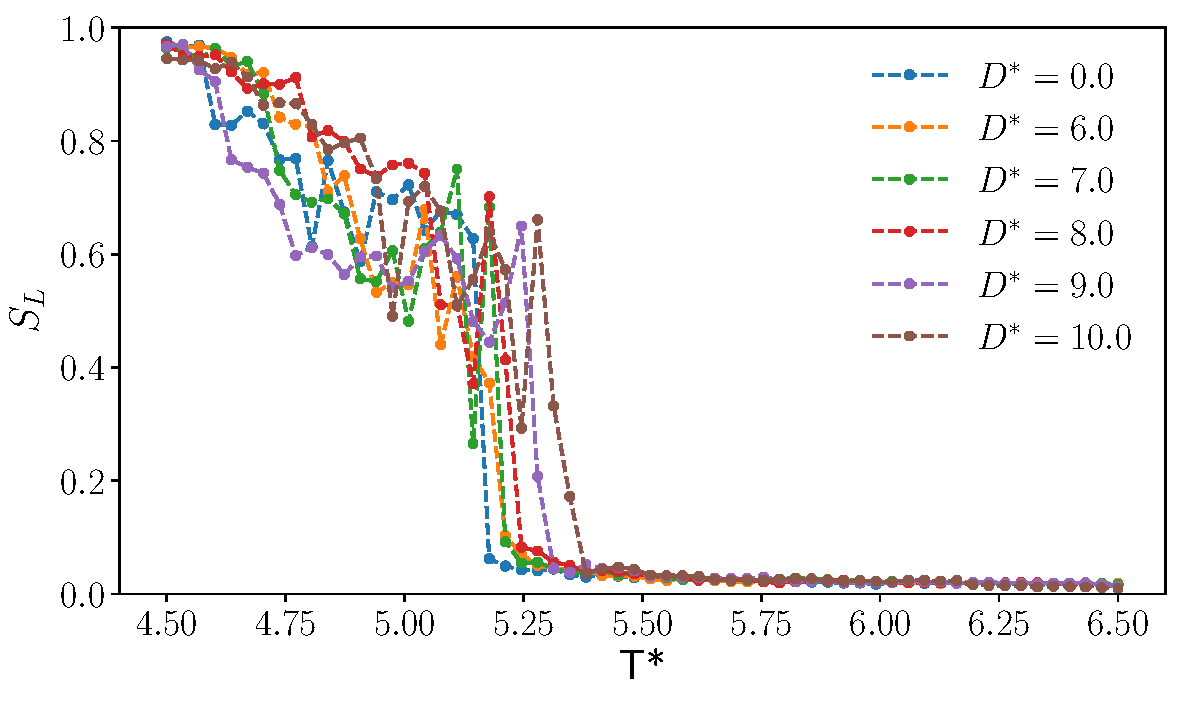
\includegraphics[width=0.7\linewidth]{plots/bfo_C32_nemsca.pdf}
	\caption{Dependence of the nematic order parameter and the hexagonal on the temperature for systems in bulk with colloids of different size}
    \label{fig:beoc32lochex}
\end{figure}


\subsubsection{Potential strength $\epsilon_{\text{cf}}= 80\epsilon_{\text{ff}}$}
Increasing the potential to $\epsilon_{\text{cf}}= 80\epsilon_{\text{ff}}$ we see more substantial results. For smaller colloid sizes ($D^*\in \{6,7,8\}$) we see no difference in the phase transition, whereas with a colloid of diameter $D^*=9.0$ the transition is shifted towards a colder temperature, and with a colloid of diameter $D^*=10.0$ the transition doesn't even appear in the probed temperature range.
\begin{figure}[H]
    \centering
	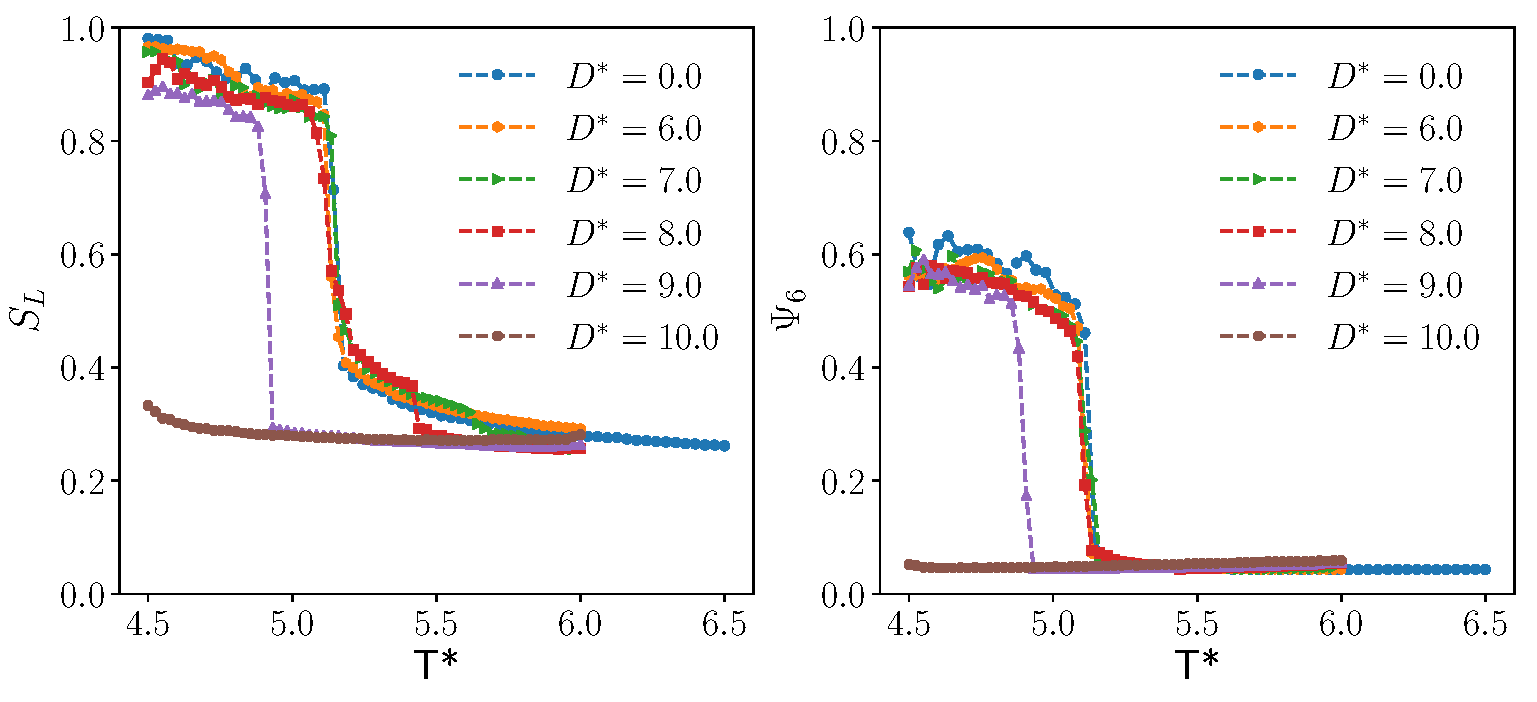
\includegraphics[width=\linewidth]{plots/bfo_C80_nemhex.pdf}
	\caption{Dependence of the local nematic order parameter and the hexagonal on the temperature for systems in bulk with colloids of different size}
    \label{fig:beoc32lochex}
\end{figure}
\begin{figure}[H]
    \centering
	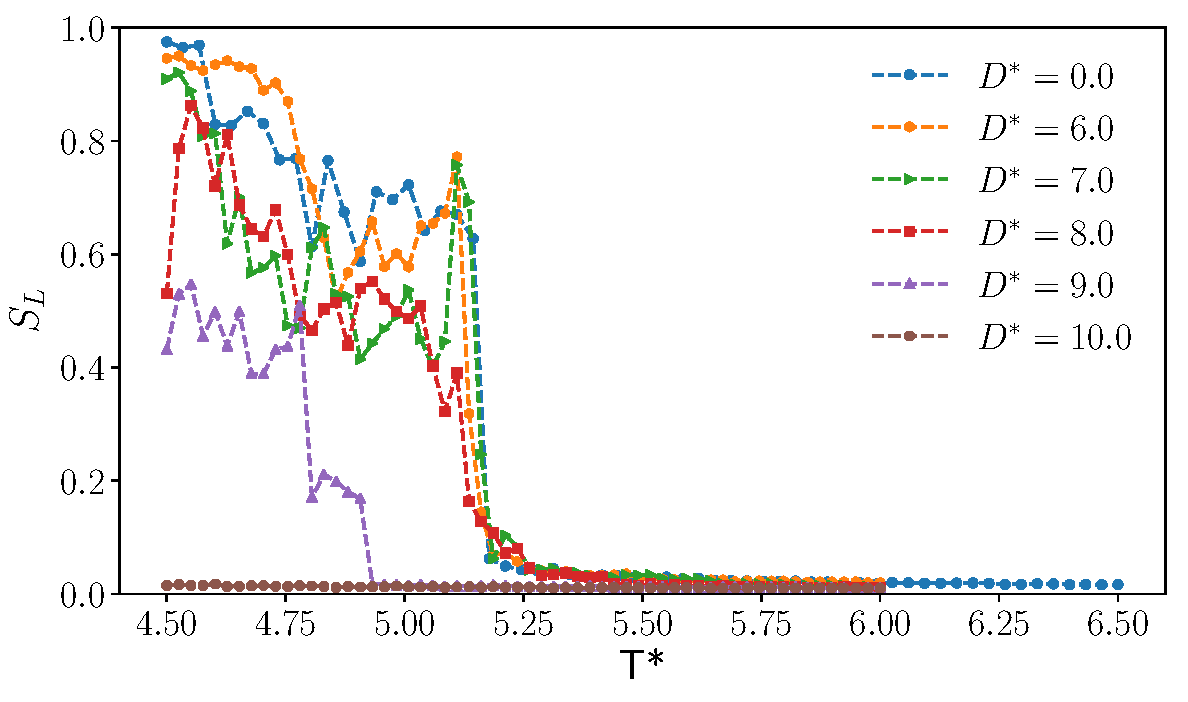
\includegraphics[width=0.7\linewidth]{plots/bfo_C80_nemsca.pdf}
	\caption{Dependence of the nematic order parameter and the hexagonal on the temperature for systems in bulk with colloids of different size}
    \label{fig:beoc32lochex}
\end{figure}

Looking at the the radial density, we can definitely see the formation of layers around the colloid, where the local bond order on these layers is lower than outside, obviously due to the impossibility of formation of radially aligned columns around the colloid.

\begin{figure}[H]
    \centering
	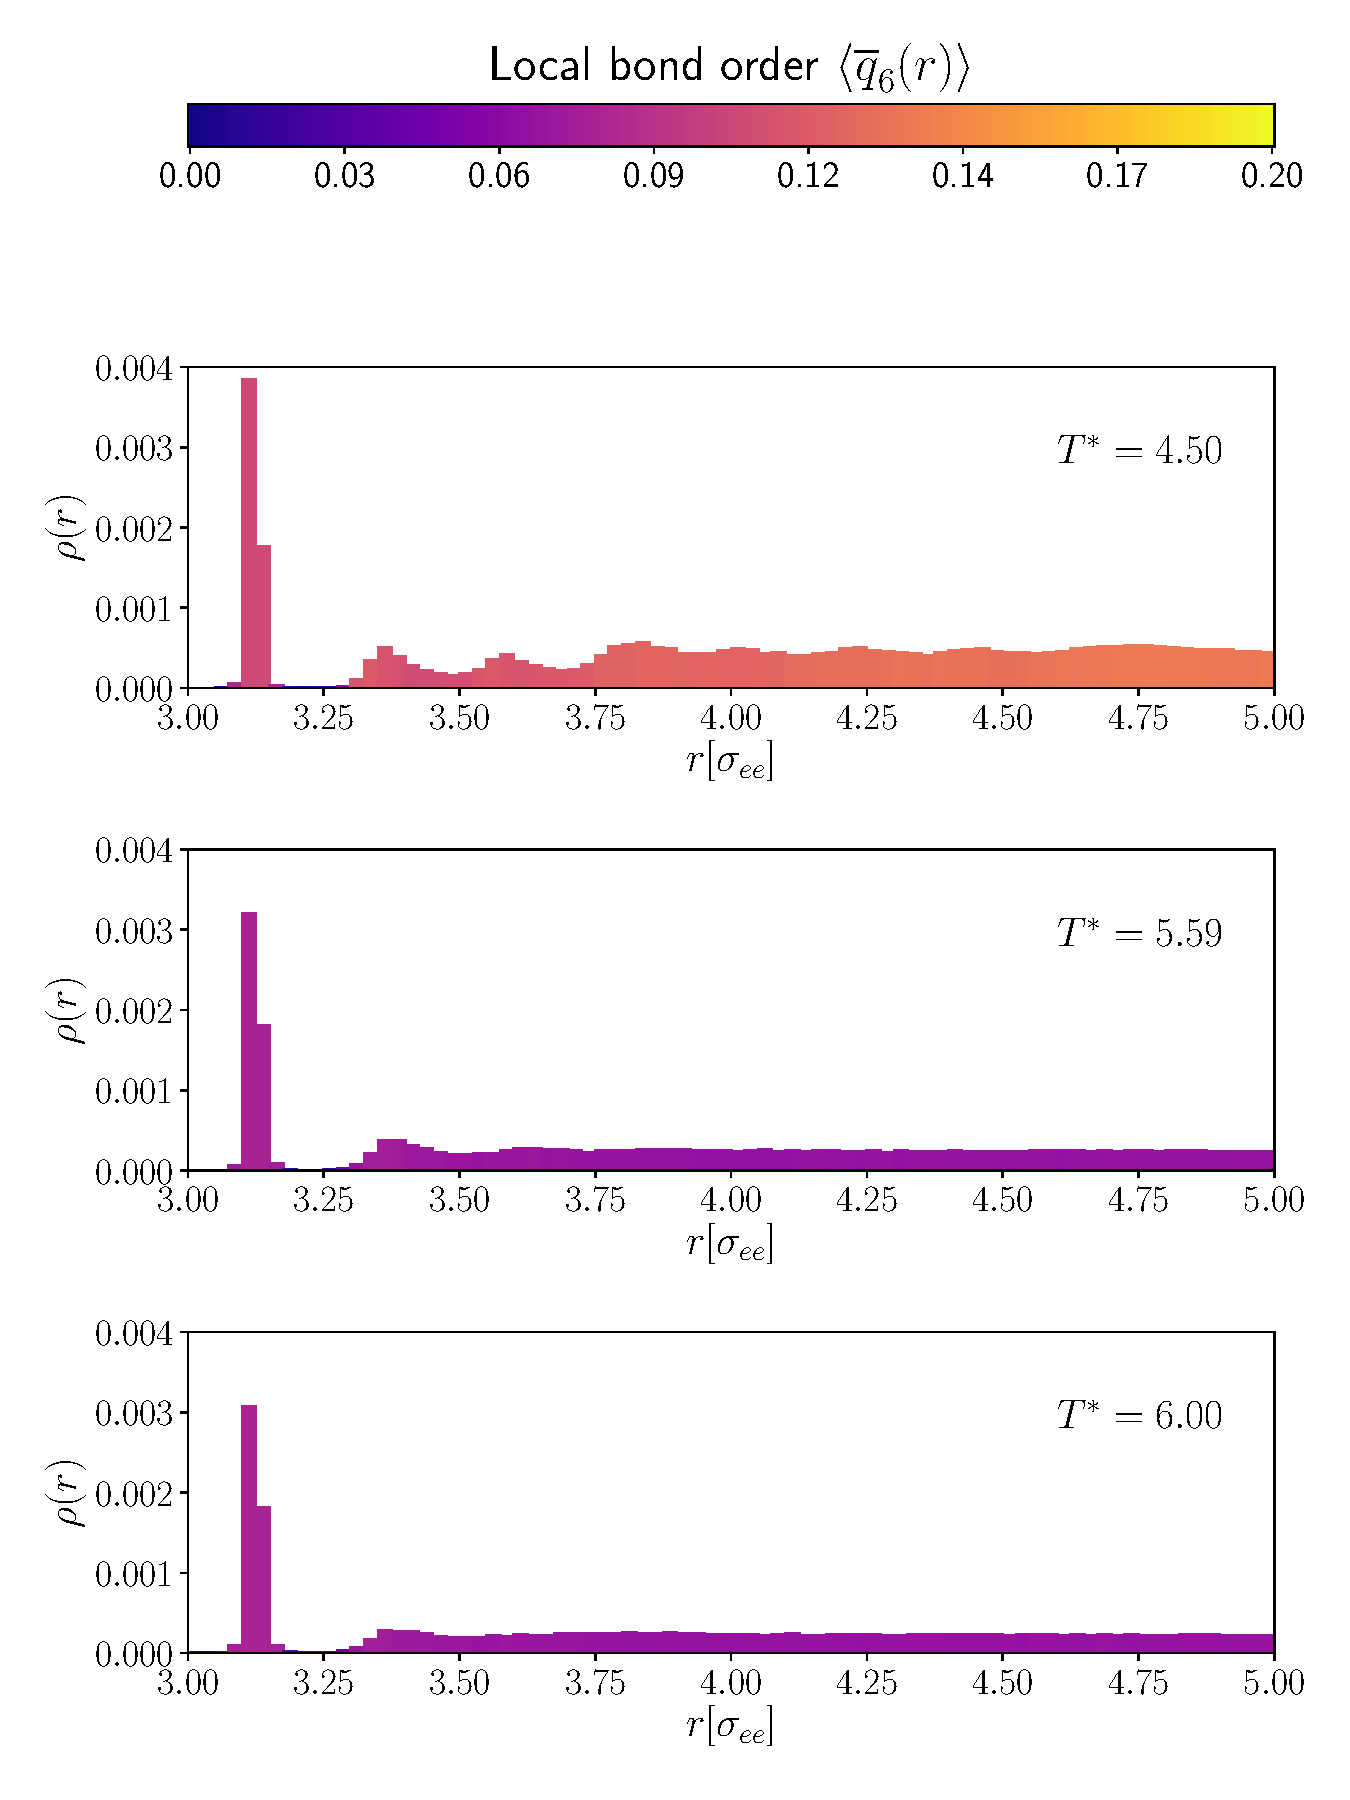
\includegraphics[width=0.49\linewidth]{plots/bfo_C80_raddensD6.pdf}
	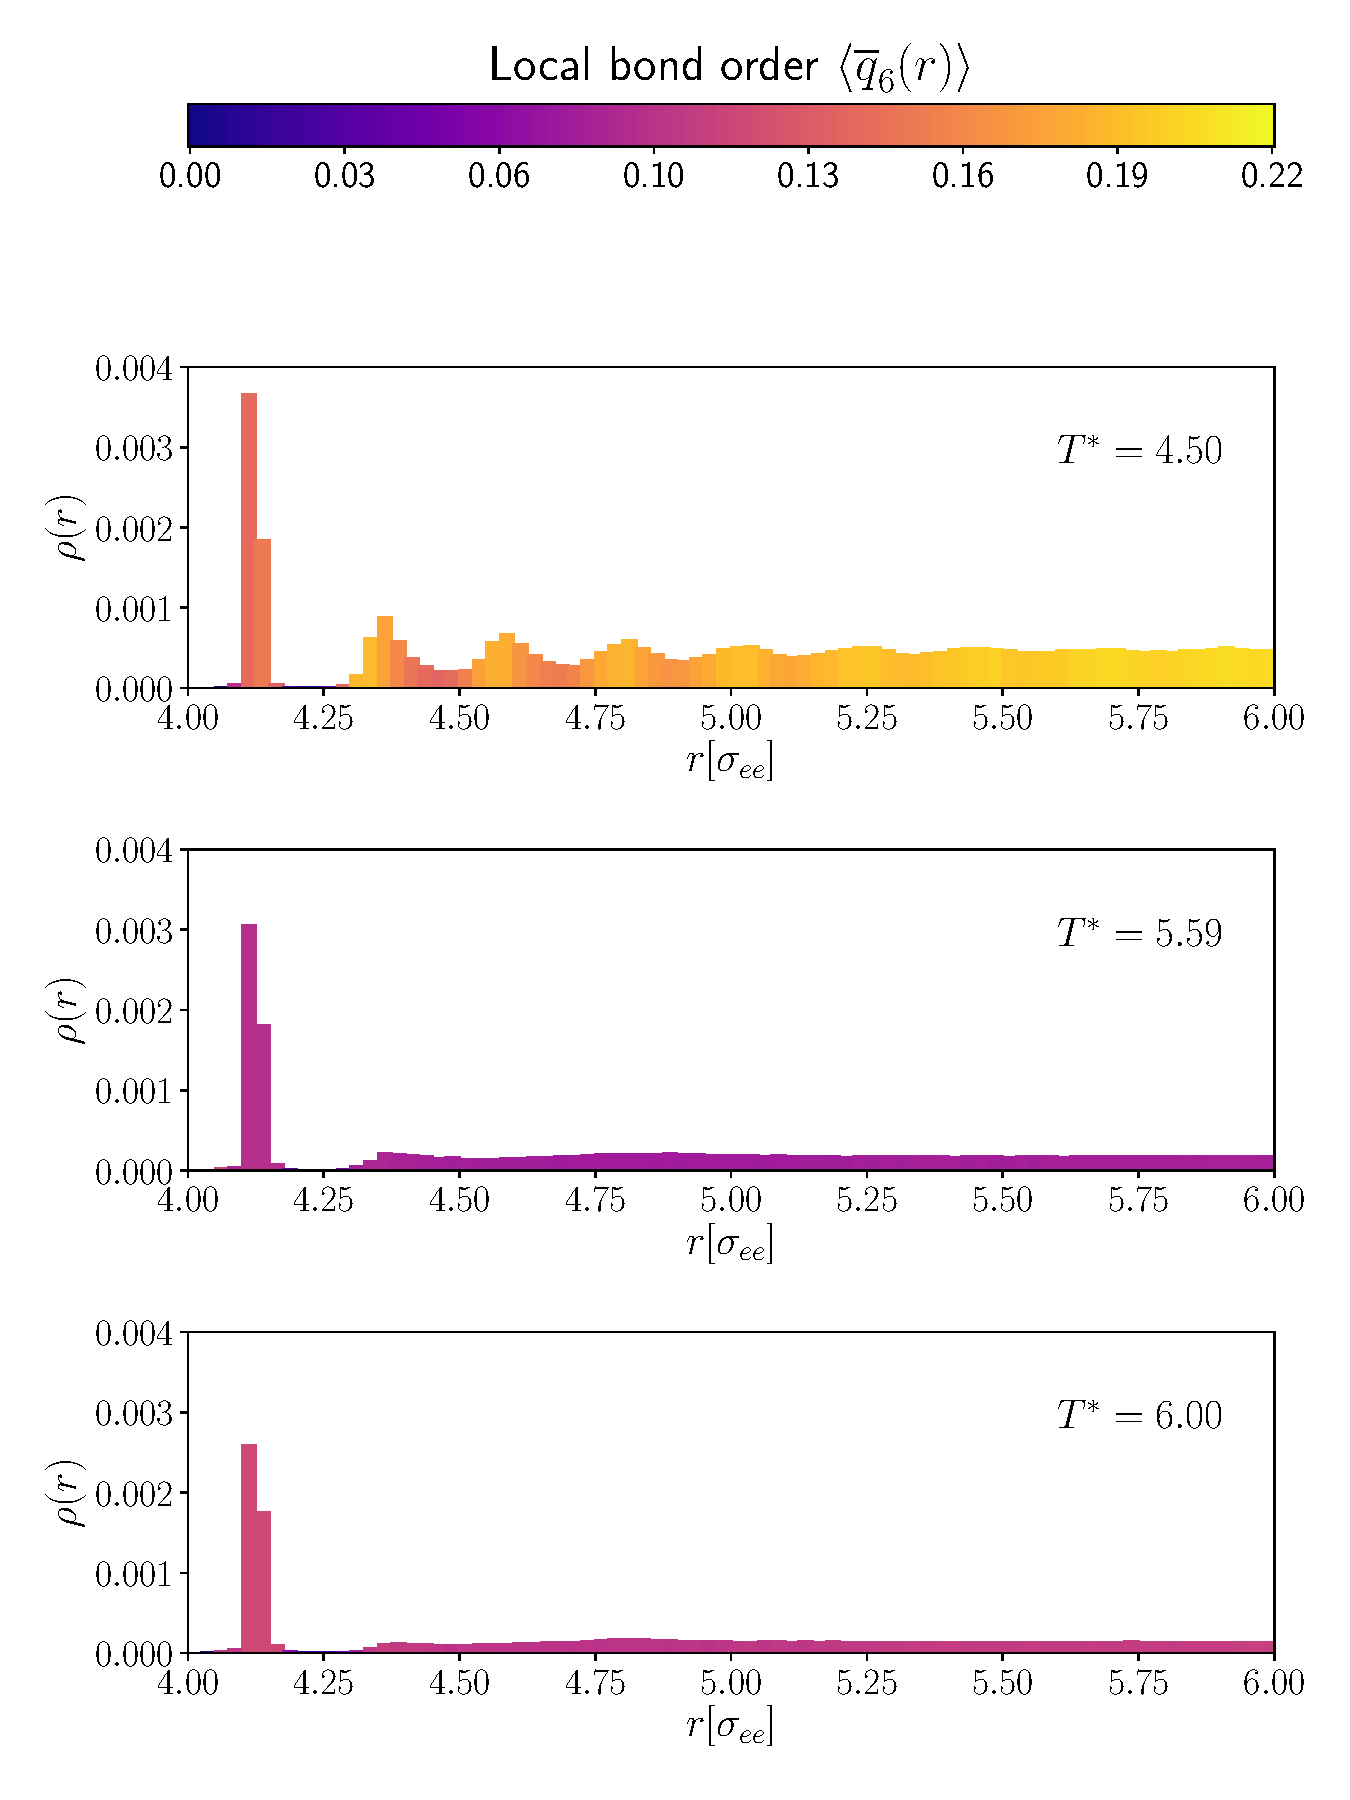
\includegraphics[width=0.49\linewidth]{plots/bfo_C80_raddensD8.pdf}
	\caption{Radial dependence of the local density and bond orientational order parameter $ \overline{q}_6$ at different temperatures for a system with a colloid of size $D^* =  6$ (left) and $D^* = 8$ (right).}
    \label{fig:beoc32nemloc}
\end{figure}


An as of now unfortunately unavoidable factor in these simulations is the small size effect, especially noticeable in Figure \ref{fig:bfosnapshots}. As mentioned in the beginning of this section, increasing the system size may increase the running time by a lot, since the more particles there are, the more steps are required to reach equilibrium. I will try to implement a non-cubic periodic unit cell and see if the improvement is significant.